%!TEX root = ../thesis.tex

\chapter{Experiments and Results}
\label{cha:experimentsandresults}

In this chapter its going to be explained the setup required to run the experiments,
the datasets used during this experiments and its numerical and qualitative results.

\section{Setup}
\subsection{Workstation}

The main developing tool has been a laptop which has been used for a huge variaty of tasks: write code, debug, check papers and documentation, write notes, etc.
In order to train and make prediciton with deep learning models, an intensive computational resources are required.

This is why in addition, access to a GPU cluster has been provided in order to train models using GPUs.
The Computer Vision Lab provide access to BIWI cluster which has been used to store datasets and models and also as a computation resource. The BIWI cluster consists on 70 computational nodes (CPU only) with a total of 556 processors, 8328 cores and 13.3TB of RAM memory.
In addition, there are the GPU nodes which consists in 75 GPUs with 12GB of GPU memory each one.

\subsection{Software}

All the code developement has been done using the Python3 language.
Python is commonly extended in computer vision and deep learning applications because all the available libraries that provides computational frameworks and also because its easiness developing.

The main library used to develop deep learning models has been PyTorch~\cite{paszke2017automatic}. This library provides high-level features for tensor computation and deep neural networks.
This library is a wrapper in Python which under the hood is writen in C allowing fast performance and strong GPU acceleration.
This library is usually used in the research community because its flexibility, fast code prototyping and easily debugging capabilities.

\section{Datasets}

During the development of this thesis, two segmentation datasets have been used: DAVIS and PASCAL.
DAVIS was used to evaluate the instance segmentation in videos while the PASCAL was used as additional data as provides a huge set of instance annotations on images.

\subsection{DAVIS Dataset}

The DAVIS Dataset~\cite{Perazzi2016,PontTuset2017} consists on a Densely Annotated Video Segmentation dataset.
It provides a curated densely annotations for object instances in video sequences.
There are two versions of the dataset: DAVIS 2016~\cite{Perazzi2016} and DAVIS 2017~\cite{PontTuset2017}.
The 2016 version provides foreground/background annotations while the 2017 provides annotations for multiple objects and instances in the foreground.
During the work done on this thesis, DAVIS 2017 version has been used.
Some examples of the annotations are shown in \figref{davis} and information about the dataset is also given in \tabref{davis}.

\begin{table}[h]
  \centering
  \begin{tabular}{l|lllll}
    DAVIS 2017                          & train & val  & test-dev & test-challenge & \textbf{Total} \\
    \hline
    Number of sequences                 & 60    & 30   & 30       & 30             & \textbf{50}    \\
    Number of frames                    & 4219  & 2023 & 2037     & 2180           & \textbf{10459} \\
    Mean number of frames per sequence  & 70.3  & 67.4 & 67.9     & 72.7           & \textbf{69.7}  \\
    Number of objects                   & 138   & 59   & 89       & 90             & \textbf{376}   \\
    Mean number of objects per sequence & 2.30  & 1.97 & 2.97     & 3.00           & \textbf{2.51}
  \end{tabular}
  \caption{Size of the DAVIS 2017 data splits: number of sequences, frames and annotated objects.}
  \label{tab:davis}
\end{table}

\begin{figure}[h]
  \centering
  \begin{subfigure}{.25\textwidth}
    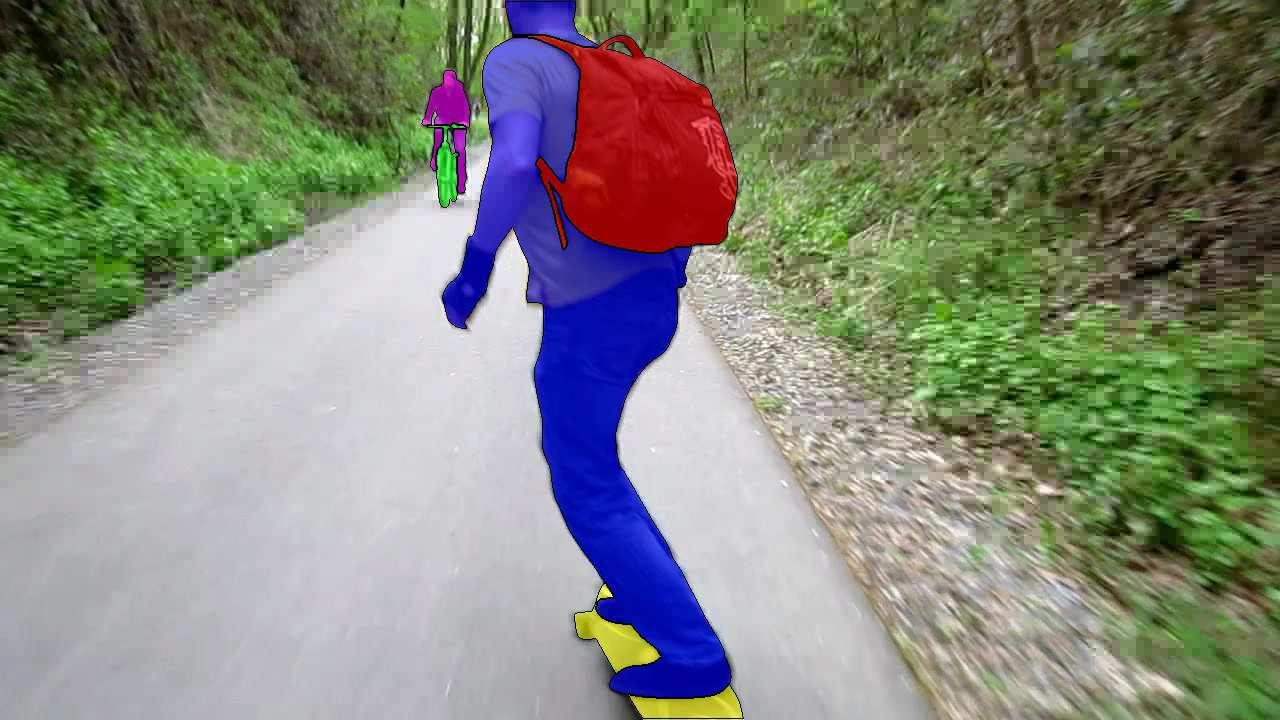
\includegraphics[width=1.\linewidth]{figures/davis_dataset/image_1.jpg}
  \end{subfigure}%
  \begin{subfigure}{.25\textwidth}
    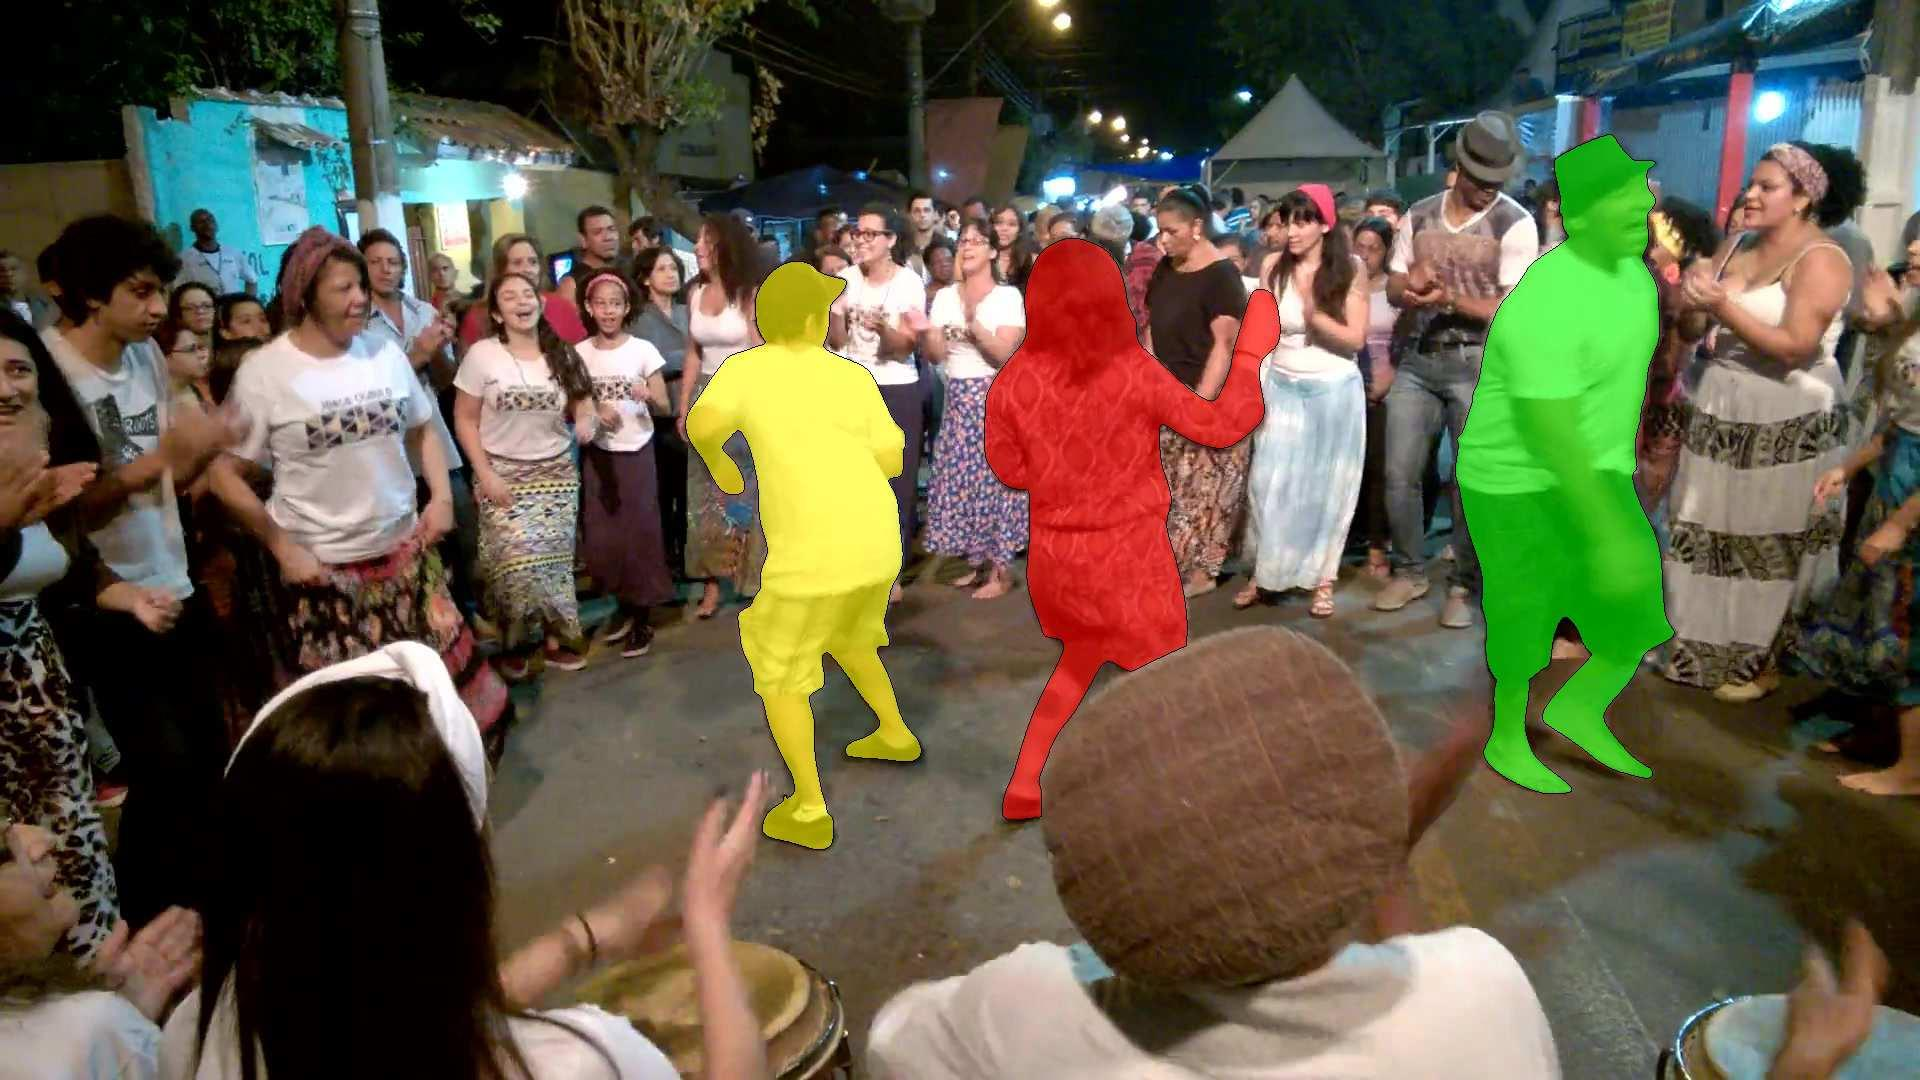
\includegraphics[width=1.\linewidth]{figures/davis_dataset/image_2.jpg}
  \end{subfigure}%
  \begin{subfigure}{.25\textwidth}
    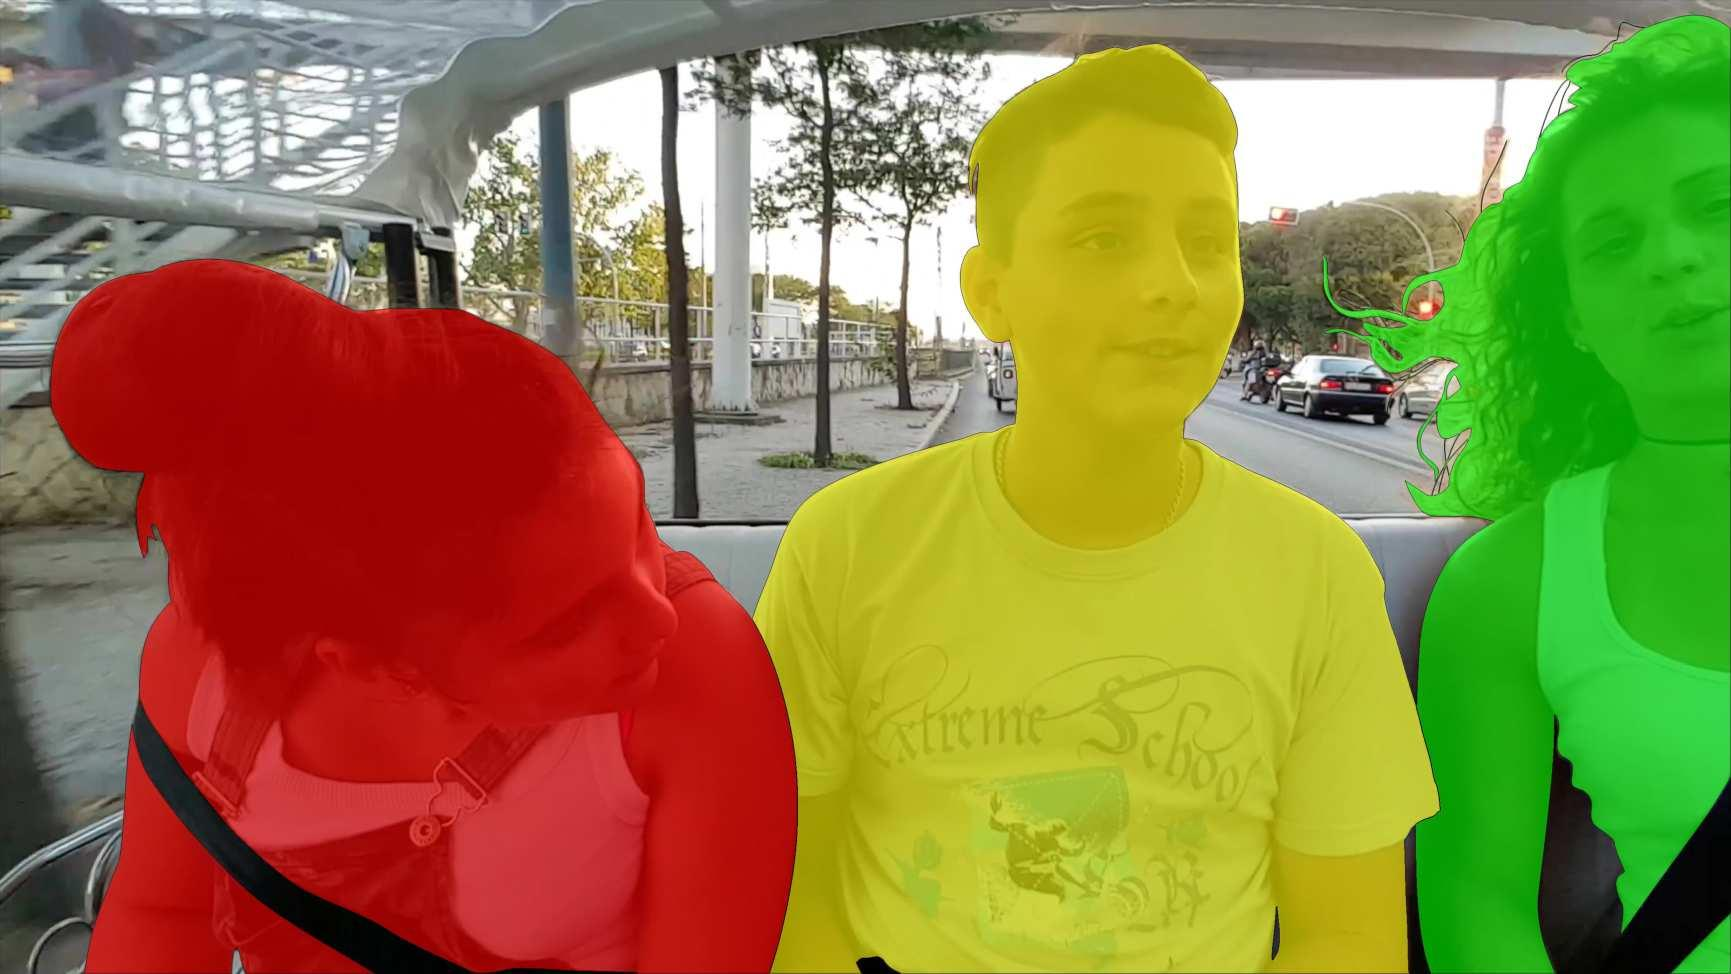
\includegraphics[width=1.\linewidth]{figures/davis_dataset/image_3.jpg}
  \end{subfigure}%
  \begin{subfigure}{.25\textwidth}
    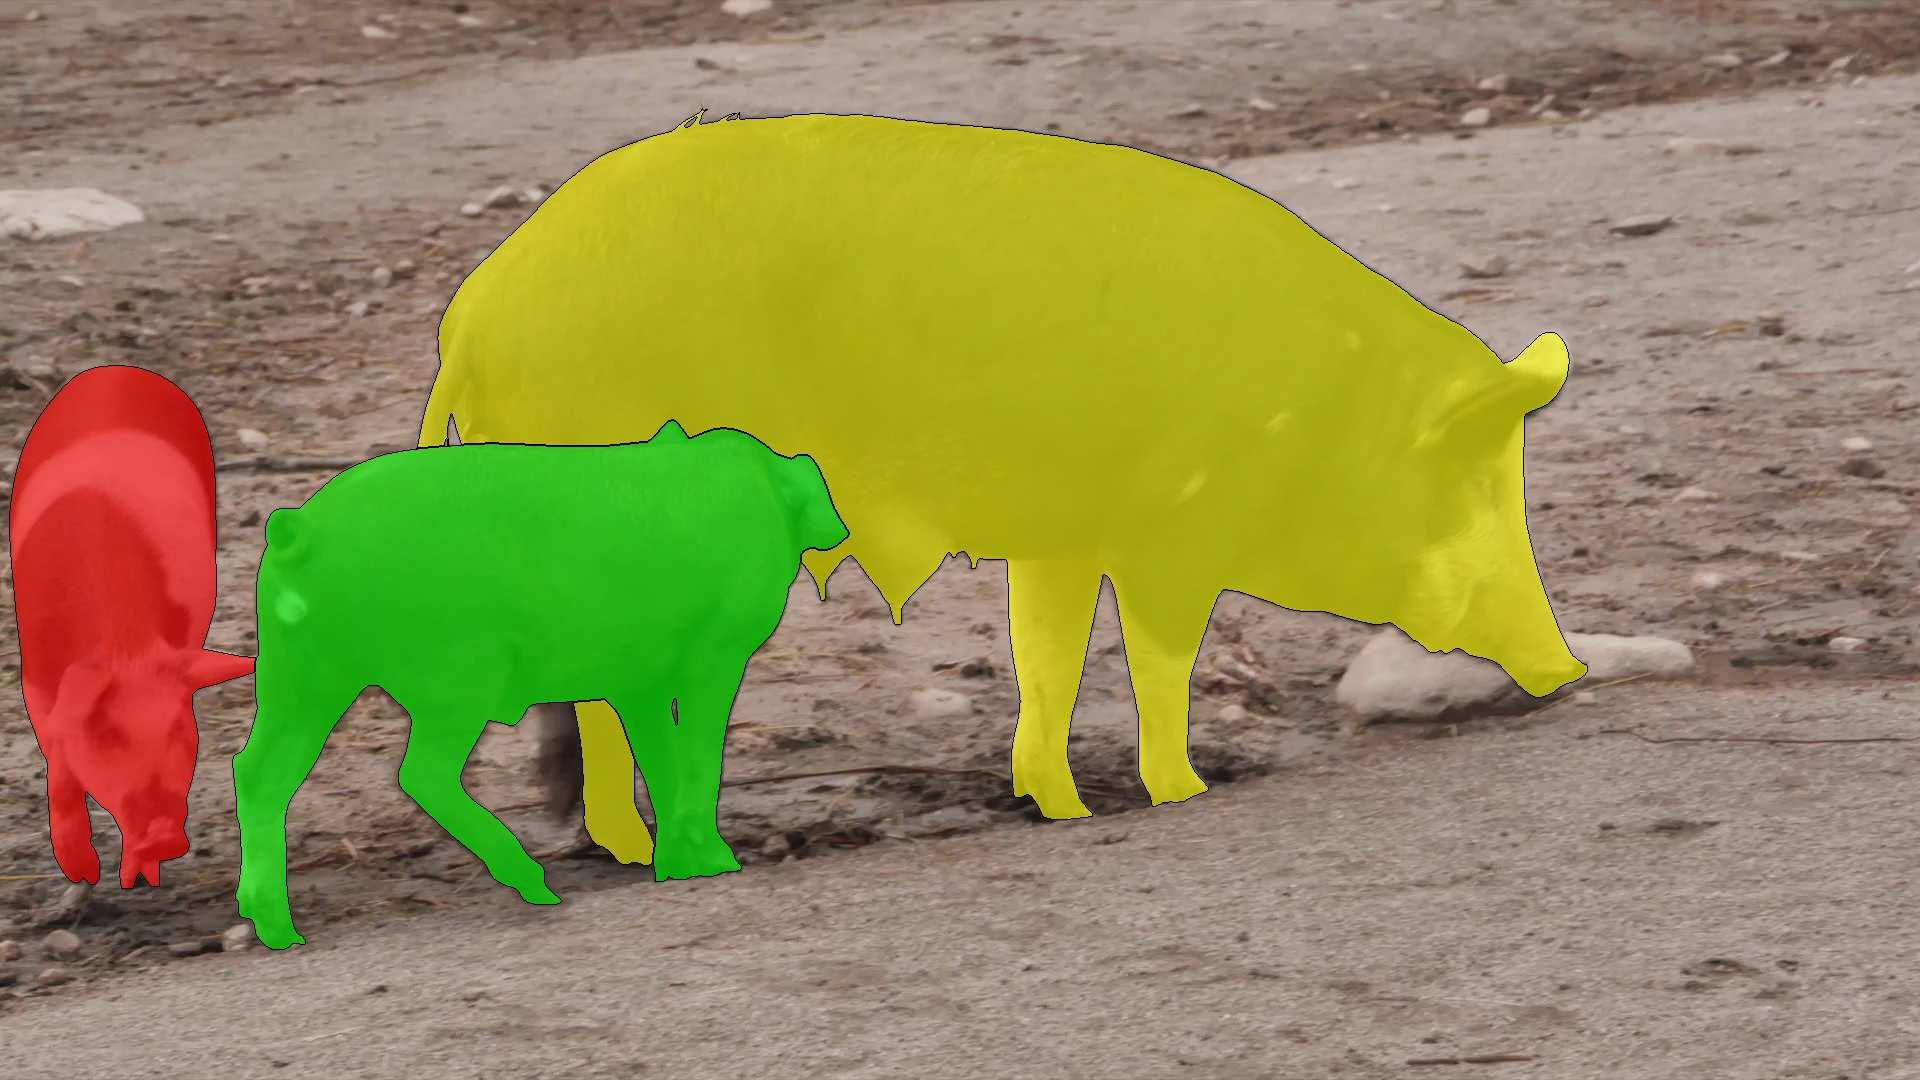
\includegraphics[width=1.\linewidth]{figures/davis_dataset/image_4.jpg}
  \end{subfigure}
  \caption{Example of annotations on DAVIS 2017 Dataset.}
  \label{fig:davis}
\end{figure}


The DAVIS dataset owners also organize a challenge to evaluate the performance of different segmentation method.
This challenge have two branches which are the following:

\paragraph{Semi-supervised}

Consists on generate a prediction given only the ground truth mask of the first frame.
This gives information to the about which is the object intended to be segmented.

\paragraph{Unsupervised}

As the name specifies, no information is given about the object that must be segmented.
To solve this, the segmentation methods rely on the frames to infer the foreground and background.

As our goal consists on weakly semi-supervised instance segmentation using tracked points, some additional annotation was required.
To obtain more data, which in this case was point trajectories inside each sequence, a manual annotation by the Segmentation Group at the Computer Vision Lab was performed.
The annotation was done using an existing tool developed inside the group by Dr. Jordi Pont-Tuset.
The annotation consisted on fixed points of the object along all the frames as well the annotation of its visibility.
An example of a fixed point in an object will be an animal's eye, a person point in the head or the center of a wheel.

\subsection{PASCAL Dataset}

PASCAL Dataset~\cite{Everingham10} is a dataset used to benchmark vision object category recognition, detections and segmentation.
Consist on images containing 20 visual object classes and provides multiple annotation for different computer vision tasks: detection and segmentation.
The segmentation annotations consist on masks over instances belonging to the 20 classes, which lead with images with multiple instance annotations.

During this thesis, the segmentation annotations from PASCAL VOC 2012 have been used. The information about the number of instances per split can be found on \tabref{pascal} and some samples of the dataset at \figref{pascal}.

\begin{table}[h]
  \centering
  \begin{tabular}{l|lll}
  PASCAL VOC 2012                    & train & val  & \textbf{Total} \\
  \hline
  Number of images                   & 1464  & 1449 & \textbf{2913}  \\
  Number of instances                & 3507  & 3427 & \textbf{6934}  \\
  Mean number of instances per image & 2.40  & 2.37 & \textbf{2.38}  \\
  \end{tabular}
  \caption{Size of the PASCAL VOC 2012 data splits: number of images and annotated objects.}
  \label{tab:pascal}
\end{table}


\begin{figure}[h]
  \centering
  % Images
  \begin{subfigure}{.25\textwidth}
    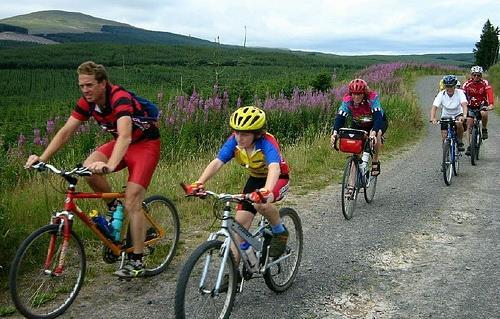
\includegraphics[width=1.\linewidth,height=0.618\linewidth]{figures/pascal_dataset/image-1.jpg}
  \end{subfigure}%
  \begin{subfigure}{.25\textwidth}
    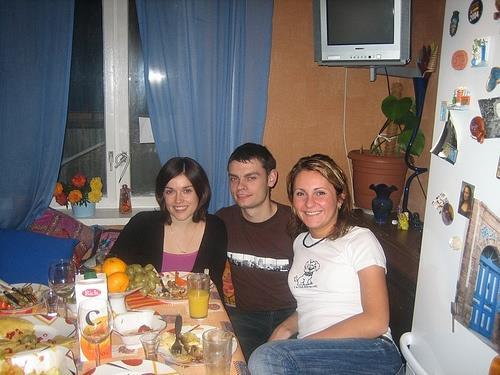
\includegraphics[width=1.\linewidth,height=0.618\linewidth]{figures/pascal_dataset/image-2.jpg}
  \end{subfigure}%
  \begin{subfigure}{.25\textwidth}
    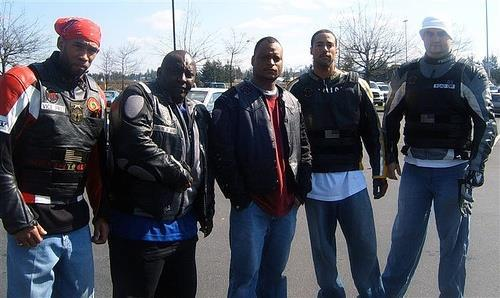
\includegraphics[width=1.\linewidth,height=0.618\linewidth]{figures/pascal_dataset/image-3.jpg}
  \end{subfigure}%
  \begin{subfigure}{.25\textwidth}
    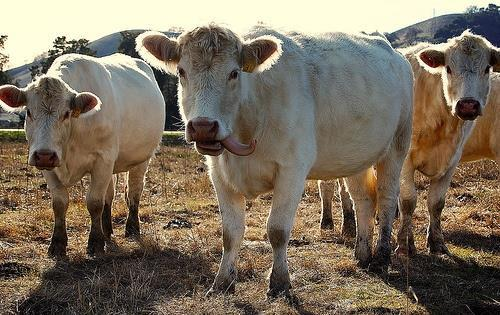
\includegraphics[width=1.\linewidth,height=0.618\linewidth]{figures/pascal_dataset/image-4.jpg}
  \end{subfigure}
  % Annotations
  \begin{subfigure}{.25\textwidth}
    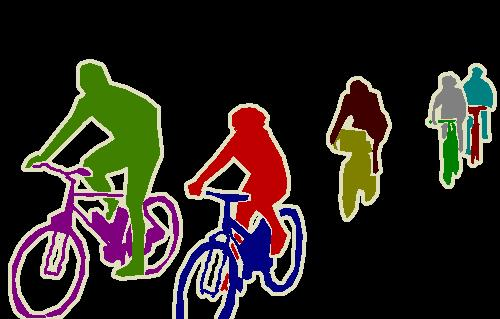
\includegraphics[width=1.\linewidth,height=0.618\linewidth]{figures/pascal_dataset/annotation-1.jpg}
  \end{subfigure}%
  \begin{subfigure}{.25\textwidth}
    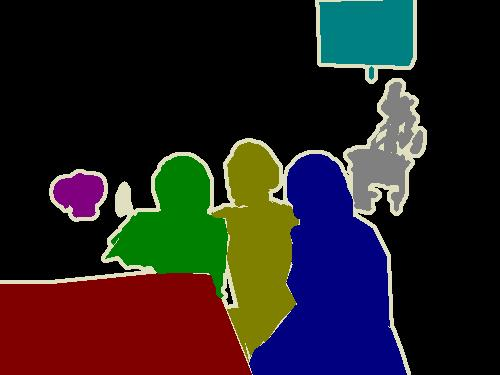
\includegraphics[width=1.\linewidth,height=0.618\linewidth]{figures/pascal_dataset/annotation-2.jpg}
  \end{subfigure}%
  \begin{subfigure}{.25\textwidth}
    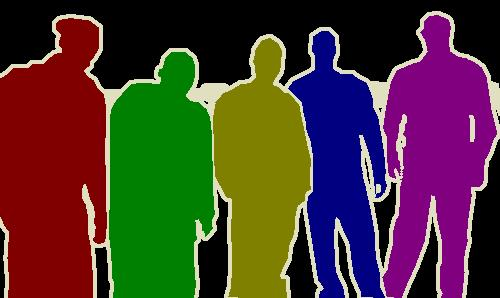
\includegraphics[width=1.\linewidth,height=0.618\linewidth]{figures/pascal_dataset/annotation-3.jpg}
  \end{subfigure}%
  \begin{subfigure}{.25\textwidth}
    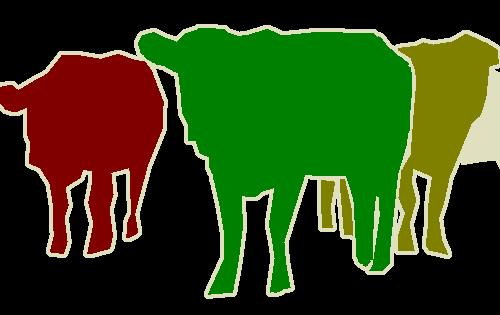
\includegraphics[width=1.\linewidth,height=0.618\linewidth]{figures/pascal_dataset/annotation-4.jpg}
  \end{subfigure}
  \caption{Example of images (top) and annotations (bottom) on PASCAL VOC 2012 Dataset.}
  \label{fig:pascal}
\end{figure}


%%%%%%%%%%%%%%%%%%%%%%%%%%%%%%%%%

\section{Experiments}

To test our proposed method we divide the experimentation in three steps.
The first step consist in test the tracking of the points.
The second one will consist on instance segmentation, once given a point belonging to an instance.
The last step consists in evaluate on video sequences the weakly semi-supervised method for video instance segmentation.

\subsection{Tracking}

In order to perform tracking of single points in video sequences we have performed two approaches.
The first approach is inspired by OSVOS~\cite{caelles2017one} work where a model is finetuned per each sequence with the information of the first frame available.
In our case the point representation as a heatmap is being used and tested against the DAVIS 2017 validation subset.

% TODO: define metric
Before presenting the results some metric should be defined.
For point tracking PCK metric can be used as it has been widely used in pose estimation to evaluate keypoint position prediction~\cite{sapp2013modec}.
This metric plots for a range of distance in pixels in the original resolution of the image (480p in our case) the detection rate. The detection rate can be seen as the percentage of samples that the prediction is as furthest the distance in pixels.


% TODO: Comment training parameters (learning rate, ...)
For the following experiments a ResNet50 backbone architecture has been used with a PSP module~\cite{zhao2017pyramid} plug at the end.
No major diference was observing using ResNet101 architecture so ResNet50 was mainly used because of its lower training time as it has less parameters to train.
The image data was fed to the model at the resolution of $512 \times 896$ pixels.
As training parameters, an SGD optimizer was used with a learning rate of $10^{-6}$, momentum $0.9$ and weight decay $0.0005$. The training for each sequence consisted on 3000 iterations with batch size $2$.

% TODO: Define Baseline and define MDNET experiments.
To compare our results, we set two baselines to compare with.
The first one consist on a single baseline where the predicted point at each frame of the sequence is the same as the point given at the first frame.
The second baseline consisted on running the MDNet~\cite{nam2016learning} tracker on the smallest bounding box that fit the ground truth mask of the sequence. The testing was performed comparing the center of the predicted bounding box against the ground truth bounding box.

% TODO: Results of tracking point regressing a heatmap for his location.
We tested two variations of the model. The first one using a single channel prediction trained with a heatmap of $\sigma = 40$ pixels.
The second variation consisted in a multiscale heatmap. In the experiment we trained using three channels with a heatmap each one of $\sigma$ equals to 24, 48 and 96 respectively.
The prediction of the point at all time was performed computing the position of the maximum value and in the case of the last variation, all the three channels were summed along the channel dimension before predicting the point position. The results are ploted on \figref{tracking_point_regression}.

\begin{figure}[h]
	\centering
	%!TEX root = ../thesis.tex

\begin{tikzpicture}
  \begin{axis}[
      set layers,
      width=\textwidth,
      height=.5\textwidth,
      width=\linewidth, % Scale the plot to \linewidth
      grid=both,
      grid style=dotted,
      minor ytick={0,0.05,...,1.1},
      ytick={0,0.1,...,1.1},
      yticklabels={0,.1,.2,.3,.4,.5,.6,.7,.8,.9,1},
      ymin=0, ymax=1,
      xmin=0, xmax=50,
      xlabel=Distance (pixels), % Set the labels
      ylabel=Detection Rate,
      legend columns=1,
      %transpose legend,
      cycle list name=exotic,
      legend pos= south east,
      legend style={/tikz/every even column/.append style={column sep=3mm}},
      % legend style={at={(0.5,-0.2)},anchor=north},
      % x tick label style={rotate=90,anchor=east}
    ]
    \addplot+[smooth, cyan, mark=none, line width=1]
    table [x=Threshold, y=Baseline, col sep=comma] {data/precission_threshold_curves.csv};
    \addlegendentry{Baseline}

    \addplot+[smooth, red, mark=none, line width=1]
    table [x=Threshold, y=MDNet, col sep=comma] {data/precission_threshold_curves.csv};
    \addlegendentry{MDNet}

    % \addplot+[smooth, green, mark=none, line width=1]
    % table [x=Threshold, y=Hourglass w/o Parent Network 1HG x2 sigma 5, col sep=comma] {data/precission_threshold_curves.csv};
    % \addlegendentry{Hourglass}

    % \addplot+[smooth,  mark=none, line width=1]
    % table [x=Threshold, y=ResNet101 sigma20, col sep=comma] {data/precission_threshold_curves.csv};
    % \addlegendentry{ResNet101}

    \addplot+[smooth,  mark=none, line width=1]
    table [x=Threshold, y=ResNet50 sigma40, col sep=comma] {data/precission_threshold_curves.csv};
    \addlegendentry{ResNet50}

    \addplot+[smooth,  mark=none, line width=1]
    table [x=Threshold, y=ResNet50 Multiscale sigma964824, col sep=comma] {data/precission_threshold_curves.csv};
    \addlegendentry{ResNet50 Multiscale}

  \end{axis}
\end{tikzpicture}

  \label{fig:tracking_point_regression}
	\caption{Precission performance for point regression.}
\end{figure}

%TODO:
In addition to this metric, in order to see if our model has been able to learn the representation of the object to track, we compute the a coverage factor.
This coverage factor is defined as the accuracy of the model to predict a tracked point inside the ground truth mask of the object to track.
These results are showed at \tabref{coverage_tracking_heatmap}.

\begin{table}[h]
  \centering
  \begin{tabular}{l|l}
    \toprule
    Method              & Coverage       \\
    \midrule
    Baseline            & 0.428          \\
    MDNET               & 0.851          \\
    % Hourglass           & 0.812    \\
    % ResNet101           & 0.912 \\
    ResNet50            & 0.912          \\
    ResNet50 Multiscale & \textbf{0.940} \\
    \bottomrule
  \end{tabular}
  \caption{Coverage for different methods that regress the heatmap. }
  \label{tab:coverage_tracking_heatmap}
\end{table}

%TODO:
This experiments presents good results in localization precission and coverage (at least we know that if the tracked point is not precise is consistent with the object to track.)
The big setback is regarding the training model. We need to train a model per each sequence which may leed to a big prediction time for new sequences (for the order of 10-30 minutes per sequence).

For this main reason and in order to obtain a single model to be not dependent to the sequence to track we try using unsupervised learning via metric learning. This is the second approach we tried.
Given the ResNet model, we tested this architecture with a pre-trained weights, performing some training with the triplet loss and expanding this acrhitecture with a convolutional head to reduce the embedding dimensions.

The training was performed using Adagrad optimizer with learning rate 0.001 for 100 epochs over PASCAL dataset with batch size 8. The triplet loss margin was set to $\alpha = 0.7$ and 64 triplets were sampled per image.
It was tested with the original embedding ($D=2048$) and adding a convolutional head to reduce its dimensionality.
$D=128$ was the dimensionality that presented better results. For this experiments the backbone architecture used was ResNet101 as was the only one available with pretrained weights on Video Object Classes.


\begin{figure}[h]
  \centering
  %!TEX root = ../thesis.tex

\begin{tikzpicture}
  \begin{axis}[
      set layers,
      width=\textwidth,
      height=.5\textwidth,
      width=\linewidth, % Scale the plot to \linewidth
      grid=both,
      grid style=dotted,
      minor ytick={0,0.05,...,1.1},
      ytick={0,0.1,...,1.1},
      yticklabels={0,.1,.2,.3,.4,.5,.6,.7,.8,.9,1},
      ymin=0, ymax=1,
      xmin=0, xmax=50,
      xlabel=Distance (pixels), % Set the labels
      ylabel=Detection Rate,
      legend columns=1,
      %transpose legend,
      cycle list name=exotic,
      legend pos= north west,
      legend style={/tikz/every even column/.append style={column sep=3mm}},
      % legend style={at={(0.5,-0.2)},anchor=north},
      % x tick label style={rotate=90,anchor=east}
    ]

    % \addplot+[smooth,  mark=none, line width=1]
    %   table [x=Threshold, y=Features Metric Learning Quadplet Loss (480p) Basic metriccosine patchsize3, col sep=comma] {data/precission_threshold_curves.csv};
    % \addlegendentry{Double Triplet Loss D=2048}

    \addplot+[smooth,  mark=none, line width=1]
      table [x=Threshold, y=Features Metric Learning Triplet Loss (480p) D128 Basic metriccosine patchsize3, col sep=comma] {data/precission_threshold_curves.csv};
    \addlegendentry{Triplet Loss D=128}

    \addplot+[smooth,  mark=none, line width=1]
      table [x=Threshold, y=Features Metric Learning (480p) Basic metriccosine patchsize3, col sep=comma] {data/precission_threshold_curves.csv};
    \addlegendentry{Triplet Loss D=2048}

    \addplot+[smooth,  mark=none, line width=1]
    table [x=Threshold, y=Features ResNet Basic metriccosine patchsize3, col sep=comma] {data/precission_threshold_curves.csv};
    \addlegendentry{Pre-Trained VOC D=2048}

    \addplot+[smooth,  mark=none, line width=1]
    table [x=Threshold, y=Baseline, col sep=comma] {data/precission_threshold_curves.csv};
    \addlegendentry{Baseline}

  \end{axis}
\end{tikzpicture}

  \label{fig:tracking_metric_learning}
  \caption{Precission performance for pixel representation tracking.}
\end{figure}

%TODO:
As can be seen on \figref{tracking_metric_learning} the localization precission is really poor, even in comparison with the previous experiments.
In contrast, the coverage results available in \tabref{coverage_tracking_metric_learning} increase as long as training is being performed and the dimensionality is being reduced achieving in the last configuration almost the same result with a dedicated network for each sequence.
Note that this evaluation is performed on DAVIS validation while the trained model has not seen any information from this dataset as it has been trained with the PASCAL dataset.


\begin{table}[h]
  \centering
  \begin{tabular}{l|l}
    \toprule
    Method                   & Coverage       \\
    \midrule
    Baseline                 & 0.428          \\
    Pre-Trained VOC $D=2048$ & 0.620          \\
    Triplet Loss $D=2048$    & 0.750          \\
    Triplet Loss $D=128$     & \textbf{0.911} \\
    % Double Triplet Loss $D=2048$ & 0.885    \\
    \bottomrule
  \end{tabular}
  \caption{Coverage for different tracking methods trained with metric learning. }
  \label{tab:coverage_tracking_metric_learning}
\end{table}

From this model trained using the triplet loss, we can conclude that the embeddings obtained for each pixel are representative for the instance the pixels belongs but not much from the specific point of the objet.
Even though the tracking performance is not good enought, we think that the good coverage and the good embedding quality can make this architecture valid for both tracking and segmentation using a single model which is sequence independent.
That is the reason why we move forward with this approach on the coming experiments.



%%%%%%%%%%%%%%%%%%%%%%%%%%%%%%%%%%%%%%%%%%%%%%%%
\subsection{Instance Segmentation}

% TODO:
We apply also this metric learning to obtain a segmentation from the embeddings in addition to tracking.

\begin{table}[h]
  \centering
  \begin{tabular}{r|ccccccc}
    \toprule
    Margin $\alpha$ & $.5$ & {$\mathbf{.7}$ & $.8$ & $1.0$ & $1.2$ & $1.5$ & $2.0$ \\
    \midrule
    $mIoU$ & .6351$$ & $\mathbf{.6464}$ & $.6385$ & $.5620$ & $.5825$ & $.4834$ & $.3977$ \\
    \bottomrule
  \end{tabular}
  \caption{Mean intersection over union agains the triplet Loss margin $\alpha$ used to train (ResNet101 with convolution head and $D=128$). }
  \label{tab:margin_miou}
\end{table}


% TODO:
Define metric, which is mIoU or Jaccard (there are the same).

% TODO:
Show some graphical results PCA of embeddings.

\begin{figure}[h]
  \centering
  \showpascalpca{2007_000042}
  \showpascalpca{2007_000129}
  \showpascalpca{2007_000464}
  \showpascalpca{2007_001239}
  \showpascalpca{2007_005331}
  \showpascalpca{2008_007273}
  \showpascalpca{2009_002539}
  % \showpascalpca{2009_005219}
  \showpascalpca{2010_002868}

  \caption{PCA Embeddings}
  \label{}

\end{figure}

% TODO:
Show some results from the segmentation method (thresholding distance function).

\begin{figure}[h]
  \centering

  \showpascaldistancemap{2007_005331}
  \showpascaldistancemap{2007_001239}
  \showpascaldistancemap{2007_006698}

  \caption{Distance maps}
  \label{}
\end{figure}

% TODO:
Show experiments playing with the margin of the triplet loss in order to obtain the segmentation.



%%%%%%%%%%%%%%%%%%%%%%%%%%%%%%%%%%%%%%5
\subsection{Video Instance Segmentation}


% TODO:
Last results will be from the tracking points at DAVIS segmenting using as keypoint the gt, the first frame keypoint or the tracked keypoint.

\begin{table}[h]
  \centering
  \begin{tabular}{l|l}
    \toprule
    Method                       & mIoU  \\
    \midrule
    OnAVOS                       & 0.616 \\
    OSVOS                        & 0.566 \\
    \midrule
    Perfect Keypoints            & 0.610 \\
    First frame keypoint         & 0.426 \\
    First frame keypoint tracked & 0.432 \\
    \bottomrule
  \end{tabular}
  \caption{ }
  \label{}
\end{table}

% TODO:
show results in mIoU per sequence in val subset.

\begin{figure}[h]
  \centering

  %!TEX root = ../thesis.tex

\begin{tikzpicture}
  \centering
  \hspace{-1mm}
  \begin{axis}[
    set layers,
    height=0.4\textwidth,
    width=1\textwidth,
    ymax=1,
    ymin=0,
    xmin=0,
    xmax=31,
    ylabel={Per-sequence mIoU},
    xticklabels={car-roundabout,dog,cows,camel,blackswan,car-shadow,judo,dance-twirl,parkour,goat,loading,bike-packing,pigs,libby,breakdance,drift-straight,mbike-trick,gold-fish,motocross-jump,horsejump-high,india,lab-coat,bmx-trees,dogs-jump,scooter-black,paragliding-launch,kite-surf,soapbox,shooting,drift-chicane},
	  font=\tiny, grid=both,
	  grid style=densely dotted,
	  major grid style={white!0!black},
	  minor grid style={white!80!black},
    xticklabel shift={-4pt},
    ylabel shift={-5pt},
    legend pos = north west,
    xtick={1,...,50},
    ytick={0,0.1,...,1.01},
    yticklabels={0,.1,.2,.3,.4,.5,.6,.7,.8,.9,1},
    minor ytick={0,0.025,...,1},
    cycle list name=exotic,
    x tick label style={rotate=50,anchor=north east,text depth=-1ex},
    legend style={at={(1,1)}, anchor=north east}]

    \addplot+[mark=none, thick]
    table [x=index,y=jaccard, col sep=comma] {data/miou_sequences.csv};
    \addlegendentry{Instance Segmentation with Point Tracking}
  \end{axis}
\end{tikzpicture}

  \caption{}
  \label{}
\end{figure}


% TODO:
Show graphical results of segmentations from DAVIS dataset
